\documentclass[12pt,journal]{IEEEtran}

\usepackage[utf8]{inputenc}
\usepackage{pgfplots}
\usepackage{caption}
\usepackage{mathtools}

\begin{document}

    \title{Lineal regression with two variables}
    \author{Alejandro Salgado G}
    \maketitle

    This problem consists in predicting differents ouputs based on some examples
    that the algorithm in going to receive. \\

    \begin{equation}
        h(x) = \theta_0 + \theta_1 x
    \end{equation}

    \begin{equation}
        J(\theta_0, \theta_1) = \frac{1}{2m} \sum_{i=1}^{m} ( h(x_i)  - y_i )^2
    \end{equation}

    \begin{figure}[h]

        \centering
        \captionsetup{justification=centering}

        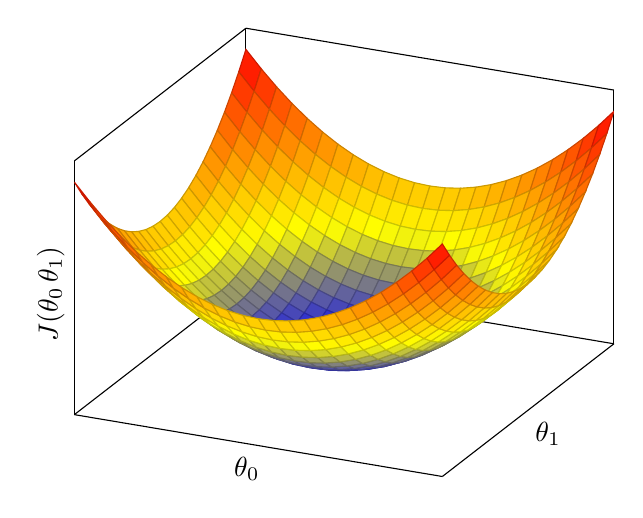
\begin{tikzpicture}
            \begin{axis}[
                            xlabel=$\theta_0$,
                            ylabel=$\theta_1$,
                            zlabel=$J(\theta_0 \, \theta_1)$,
                            xtick=\empty,
                            ytick=\empty,
                            ztick=\empty
                        ]
                \addplot3[surf]{x^2+y^2};
            \end{axis}
        \end{tikzpicture}

        \caption{Cost function}
    \end{figure}

    \begin{equation}
        \left\{
            \begin{array}{l}
                \theta_0 := \theta_0 - \alpha \Big[ \frac{\partial}{\partial \theta_0} J(\theta_0, \theta_1) \Big] \\ \\
                \theta_1 := \theta_1 - \alpha \Big[ \frac{\partial}{\partial \theta_1} J(\theta_0, \theta_1) \Big]
            \end{array}
        \right.
    \end{equation}

    lets evaluate the derivative expression of $\theta_0$ first

    \begin{equation}
        \frac{\partial}{\partial \theta_0} J(\theta_0, \theta_1)
    \end{equation}

    \begin{equation}
        \frac{\partial}{\partial \theta_0} \bigg( \frac{1}{2m} \sum_{i=1}^{m} \big[ h(x_i) - y_i\big] ^2  \bigg)
    \end{equation}

    \begin{equation}
        \frac{\partial}{\partial \theta_0} \bigg( \frac{1}{2m} \sum_{i=1}^{m} \Big[ (\theta_0 + \theta_1 x) - y_i \Big]^2  \bigg)
    \end{equation}

    \begin{equation}
        \frac{1}{2m} \sum_{i=1}^{m} \bigg( \frac{\partial}{\partial \theta_0} \Big[ (\theta_0 + \theta_1 x) - y_i \Big]^2  \bigg)
    \end{equation}

    \begin{equation}
        \frac{1}{2m} \sum_{i=1}^{m} \bigg( 2 \Big[ (\theta_0 + \theta_1 x) - y_i \Big] \frac{\partial}{\partial \theta_0} \Big[ (\theta_0 + \theta_1 x) - y_i \Big] \bigg)
    \end{equation}

    \begin{equation}
    \frac{\partial}{\partial \theta_0} \Big[ (\theta_0 + \theta_1 x) - y_i \Big]
    \end{equation}

    \begin{equation}
    \frac{\partial}{\partial \theta_0} ( \theta_0 ) + \frac{\partial}{\partial \theta_0} ( \theta_1 x ) - \frac{\partial}{\partial \theta_0} ( y_i )
    \end{equation}

    \begin{equation}
    1 + 0 - 0 = 1
    \end{equation}

    \begin{equation}
        \frac{1}{2m} \sum_{i=1}^{m} \bigg( 2 \Big[ (\theta_0 + \theta_1 x) - y_i \Big] \Big[ 1 \Big] \bigg)
    \end{equation}

    \begin{equation}
        \frac{1}{2m} \sum_{i=1}^{m} \bigg( 2 \Big[ (\theta_0 + \theta_1 x) - y_i \Big] \bigg)
    \end{equation}

    \begin{equation}
        \frac{2}{2m} \sum_{i=1}^{m} \Big( (\theta_0 + \theta_1 x) - y_i \Big)
    \end{equation}

    \begin{equation}
        \frac{1}{m} \sum_{i=1}^{m} \Big( (\theta_0 + \theta_1 x) - y_i \Big)
    \end{equation}

    \begin{equation}
        \theta_0 := \theta_0 - \alpha \Big[ \frac{1}{m} \sum_{i=1}^{m} \Big( (\theta_0 + \theta_1 x) - y_i \Big) \Big]
    \end{equation}

    For $\theta_1$ is the same exept for one step

    \begin{equation}
        \frac{\partial}{\partial \theta_1} J(\theta_0, \theta_1)
    \end{equation}

    \begin{equation}
        \frac{\partial}{\partial \theta_1} \bigg( \frac{1}{2m} \sum_{i=1}^{m} \big[ h(x_i) - y_i\big] ^2  \bigg)
    \end{equation}

    \begin{equation}
        \frac{\partial}{\partial \theta_1} \bigg( \frac{1}{2m} \sum_{i=1}^{m} \Big[ (\theta_0 + \theta_1 x) - y_i \Big]^2  \bigg)
    \end{equation}

    \begin{equation}
        \frac{1}{2m} \sum_{i=1}^{m} \bigg( \frac{\partial}{\partial \theta_1} \Big[ (\theta_0 + \theta_1 x) - y_i \Big]^2  \bigg)
    \end{equation}

    \begin{equation}
        \frac{1}{2m} \sum_{i=1}^{m} \bigg( 2 \Big[ (\theta_0 + \theta_1 x) - y_i \Big] \frac{\partial}{\partial \theta_1} \Big[ (\theta_0 + \theta_1 x) - y_i \Big] \bigg)
    \end{equation}

    \begin{equation}
    \frac{\partial}{\partial \theta_1} \Big[ (\theta_0 + \theta_1 x) - y_i \Big]
    \end{equation}

    \begin{equation}
    \frac{\partial}{\partial \theta_1} ( \theta_0 ) + \frac{\partial}{\partial \theta_1} ( \theta_1 x ) - \frac{\partial}{\partial \theta_1} ( y_i )
    \end{equation}

    \begin{equation}
    0 + x_i - 0 = 1
    \end{equation}

    \begin{equation}
        \frac{1}{2m} \sum_{i=1}^{m} \bigg( 2 \Big[ (\theta_0 + \theta_1 x) - y_i \Big] ( x_i ) \bigg)
    \end{equation}

    \begin{equation}
        \frac{2}{2m} \sum_{i=1}^{m} \bigg[ \Big( (\theta_0 + \theta_1 x) - y_i \Big) ( x_i ) \bigg]
    \end{equation}

    \begin{equation}
        \frac{1}{m} \sum_{i=1}^{m} \bigg[ \Big( (\theta_0 + \theta_1 x) - y_i \Big) ( x_i ) \bigg]
    \end{equation}

    \begin{equation}
        \theta_0 := \theta_0 - \alpha \Bigg( \frac{1}{m} \sum_{i=1}^{m} \bigg[ \Big( (\theta_0 + \theta_1 x) - y_i \Big) ( x_i ) \bigg] \Bigg)
    \end{equation}

\end{document}
